\documentclass[10pt, aspectratio=169]{beamer}

\usetheme{metropolis}
\metroset{progressbar=frametitle}
\metroset{block=fill}

% ============================================================
% UNSW Color Scheme --- YELLOW PRIMARY
% ============================================================
\definecolor{UNSWDarkBlue}{HTML}{000F2B}
\definecolor{UNSWYellow}{HTML}{FFD200}
\definecolor{UNSWRed}{HTML}{E63E30}
\definecolor{UNSWLightGray}{HTML}{F0F0F0}
\definecolor{UNSWGreen}{HTML}{00843D}

% Frame titles: yellow background, dark text
\setbeamercolor{frametitle}{bg=UNSWYellow, fg=UNSWDarkBlue}
% Title separator: dark blue
\setbeamercolor{title separator}{fg=UNSWDarkBlue}
% Progress bar: dark blue
\setbeamercolor{progress bar}{fg=UNSWDarkBlue, bg=UNSWDarkBlue!20}
\setbeamercolor{progress bar in head/foot}{fg=UNSWDarkBlue, bg=UNSWDarkBlue!20}
\setbeamercolor{progress bar in section page}{fg=UNSWDarkBlue, bg=UNSWDarkBlue!20}
% Normal text: dark blue on white
\setbeamercolor{normal text}{fg=UNSWDarkBlue, bg=white}
% Alerted text: UNSW red
\setbeamercolor{alerted text}{fg=UNSWRed}
% Palette primary (used for title slide, standout, section pages)
\setbeamercolor{palette primary}{bg=UNSWDarkBlue, fg=white}
% Block titles: dark blue bg, white text
\setbeamercolor{block title}{bg=UNSWDarkBlue, fg=white}
\setbeamercolor{block body}{bg=UNSWLightGray, fg=UNSWDarkBlue}
% Structure and itemize
\setbeamercolor{structure}{fg=UNSWDarkBlue}
\setbeamercolor{item}{fg=UNSWDarkBlue}
\setbeamercolor{section in toc}{fg=UNSWDarkBlue}

% ============================================================
% Packages
% ============================================================
\usepackage{booktabs}
\usepackage{graphicx}
\usepackage{amsmath, amssymb}
\usepackage{hyperref}
\usepackage{tikz}
\usetikzlibrary{shapes.geometric, arrows.meta, positioning, calc, fit}
\usepackage{appendixnumberbeamer}
\usepackage{pifont}
\usepackage{colortbl}
\usepackage{multirow}
\usepackage[backend=bibtex, style=numeric, maxnames=2, sorting=none]{biblatex}
\addbibresource{references.bib}

% ============================================================
% Custom commands
% ============================================================
\newcommand{\cmark}{{\color{UNSWGreen}\ding{51}}}
\newcommand{\xmark}{{\color{UNSWRed}\ding{55}}}
\newcommand{\pmark}{{\color{UNSWYellow!70!black}$\sim$}}

% Tighter itemize spacing
\setlength{\parskip}{0pt}

% ============================================================
% Metadata
% ============================================================
\title{Multi-Task Financial NLP: Stance \& Sentiment Classification of FOMC Communications and News Headlines}
\subtitle{COMP6713 --- Natural Language Processing --- 2026 T1}
\author{Louis Nguyen \and Quoc Dat Bui \and Nam Khanh Tran \and Quang Minh Phan}
\institute{UNSW School of Computer Science and Engineering}
\date{\today}

% ============================================================
\begin{document}

% ---- Title Slide ------------------------------------------
\maketitle

% ---- Outline ----------------------------------------------
\begin{frame}{Outline}
    \tableofcontents
\end{frame}

% ============================================================
\section{Problem}
% ============================================================

% ---- Two Tasks --------------------------------------------
\begin{frame}{Two Financial NLP Classification Tasks}
    We tackle \textbf{two complementary 3-class classification problems} over short financial text.

    \vspace{0.3em}
    \begin{columns}[T]
        \begin{column}{0.48\textwidth}
            \begin{block}{Stance --- FOMC Communications}
                Label the monetary-policy stance of a sentence from U.S.\ Federal Reserve meetings~\cite{shah2023trillion}.
                \begin{itemize}\setlength{\itemsep}{1pt}
                    \item \textbf{dovish} --- easing bias
                    \item \textbf{hawkish} --- tightening bias
                    \item \textbf{neutral} --- no clear bias
                \end{itemize}
                \textit{``\ldots the Committee decided to lower the target range for the federal funds rate.''} $\rightarrow$ \alert{dovish}
            \end{block}
        \end{column}
        \begin{column}{0.48\textwidth}
            \begin{block}{Sentiment --- Financial PhraseBank}
                Label the investor-facing tone of a news headline~\cite{malo2014good}.
                \begin{itemize}\setlength{\itemsep}{1pt}
                    \item \textbf{negative}
                    \item \textbf{neutral}
                    \item \textbf{positive}
                \end{itemize}
                \textit{``Operating profit totalled EUR 21.1 mn, up from EUR 18.6 mn a year earlier.''} $\rightarrow$ \alert{positive}
            \end{block}
        \end{column}
    \end{columns}
\end{frame}

% ---- Why it matters ---------------------------------------
\begin{frame}{Why It Matters}
    \begin{itemize}\setlength{\itemsep}{0.3em}
        \item \textbf{Central-bank stance moves markets.} A single sentence shift between hawkish and dovish language in an FOMC statement can reprice rates, equities, and FX within seconds.
        \item \textbf{News sentiment drives short-horizon prices.} Headline tone correlates with intraday returns and is a staple input to systematic trading and risk models.
        \item \textbf{Both tasks share domain vocabulary} but differ in pragmatics: stance is about \textit{policy direction}, sentiment is about \textit{corporate outlook}. This motivates \alert{joint modelling}.
        \item \textbf{Labelled data is scarce and expensive.} FOMC: 2{,}480 sentences; FPB allagree: 2{,}264 sentences. Techniques that squeeze more signal out of small domain corpora are essential.
        \item \textbf{Practical goal:} a single deployable encoder that does both jobs competitively.
    \end{itemize}
\end{frame}

% ============================================================
\section{Datasets}
% ============================================================

% ---- Dataset overview table -------------------------------
\begin{frame}{Dataset Overview}
    \centering
    \resizebox{\linewidth}{!}{%
    \begin{tabular}{@{}llp{3.2cm}p{4.4cm}p{3.8cm}@{}}
        \toprule
        \textbf{Name} & \textbf{Sentences} & \textbf{Classes} & \textbf{Label distribution (test)} & \textbf{Notes} \\
        \midrule
        FOMC (Trillion Dollar Words)~\cite{shah2023trillion}
            & 2{,}480 & 3 (dovish / hawkish / neutral)
            & dovish 130 (26.2\%) \newline hawkish 121 (24.4\%) \newline neutral 245 (49.4\%)
            & Sentences from FOMC statements, meeting minutes, and press conferences. Neutral-heavy. \\
        \addlinespace
        Financial PhraseBank \emph{allagree}~\cite{malo2014good}
            & 2{,}264 & 3 (negative / neutral / positive)
            & negative 61 (13.5\%) \newline neutral 278 (61.4\%) \newline positive 114 (25.2\%)
            & News headlines with 100\% annotator agreement. Highly neutral-skewed; negatives rare. \\
        \addlinespace
        Loughran--McDonald Lexicon~\cite{loughran2011liability}
            & --- & rule-based \newline (pos / neg / uncertainty)
            & pos $\approx$110 terms \newline neg $\approx$230 terms \newline uncertainty $\approx$90 terms
            & Domain financial word lists; also includes hawkish ($\approx$40) and dovish ($\approx$50) monetary-policy lists. \\
        \bottomrule
    \end{tabular}%
    }

    \vspace{0.6em}
    \begin{itemize}\setlength{\itemsep}{1pt}
        \item Short texts (mostly $< 40$ tokens) from the financial domain.
        \item FOMC and FPB are \textbf{imbalanced} with \textbf{dominant neutral}; LM Lexicon provides a domain-aware rule-based baseline and auxiliary features.
    \end{itemize}
\end{frame}

% ---- Preprocessing & splits -------------------------------
\begin{frame}{Preprocessing \& Splits}
    \begin{columns}[T]
        \begin{column}{0.54\textwidth}
            \textbf{Splits (stratified, \texttt{random\_state=42}):}
            \begin{itemize}\setlength{\itemsep}{1pt}
                \item 70\% train / 10\% validation / 20\% test
                \item FOMC: 1736 / 248 / 496
                \item FPB allagree: 1584 / 227 / 453
            \end{itemize}

            \vspace{0.3em}
            \textbf{Text normalisation:}
            \begin{itemize}\setlength{\itemsep}{1pt}
                \item Unicode NFKC, strip control chars, collapse whitespace
                \item Lower-case only for TF-IDF baselines
                \item Keep case and punctuation for BERT-family models (\texttt{max\_len}=128)
            \end{itemize}

            \vspace{0.3em}
            \textbf{Class weights for FOMC (weighted cross-entropy):}
            \[
                w_c = \frac{N}{K \cdot n_c}, \qquad
                w = (1.272,\; 1.365,\; 0.675)
            \]
            for (dovish, hawkish, neutral) with $K=3$, $N=1736$.
        \end{column}
        \begin{column}{0.42\textwidth}
            \centering
            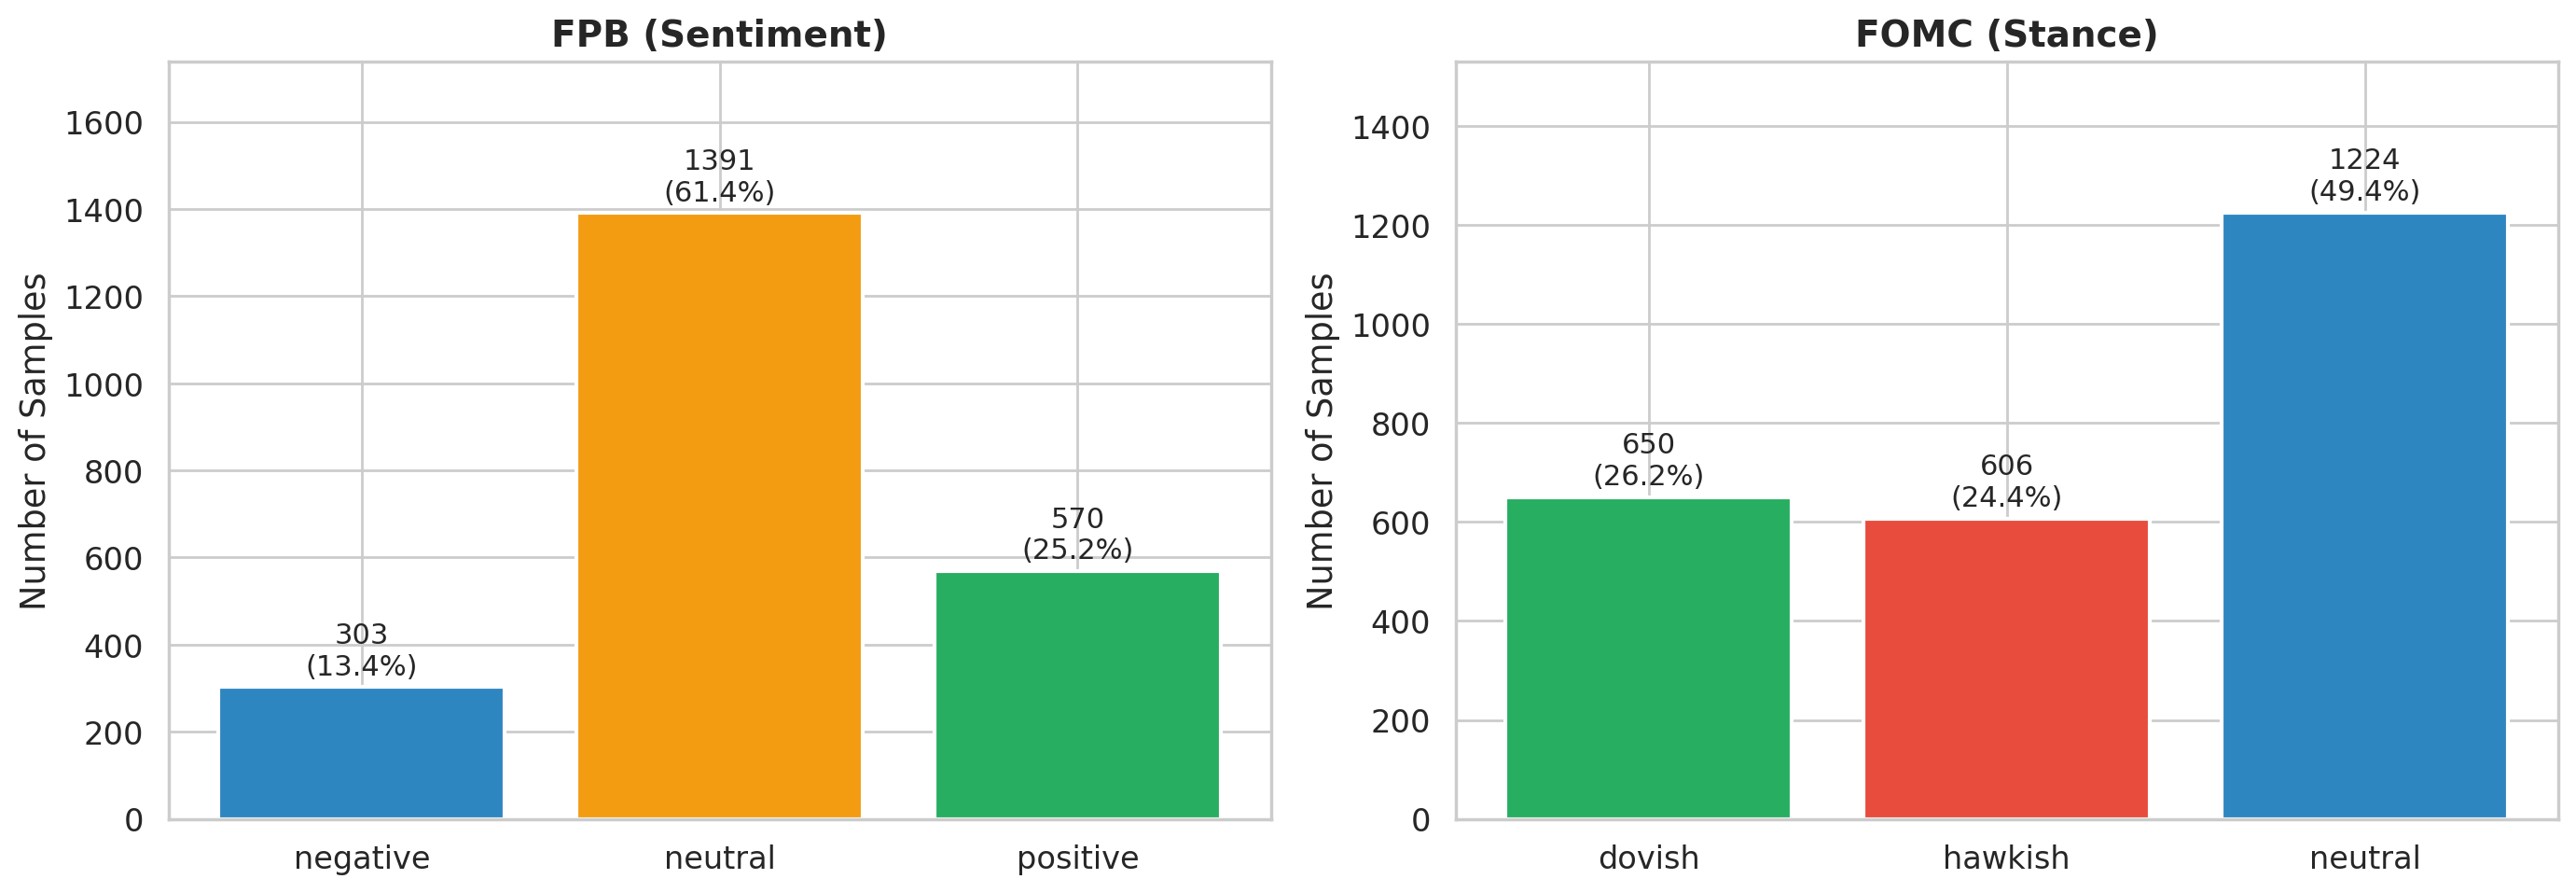
\includegraphics[width=\linewidth]{../analysis/class_distribution.png}
            {\scriptsize Class distributions for both tasks --- neutral dominates in both, negatives and hawkish labels are the minority classes.}
        \end{column}
    \end{columns}
\end{frame}

% ============================================================
\section{Methodology}
% ============================================================

% ---- Pipeline overview ------------------------------------
\begin{frame}{Pipeline Overview}
    \centering
    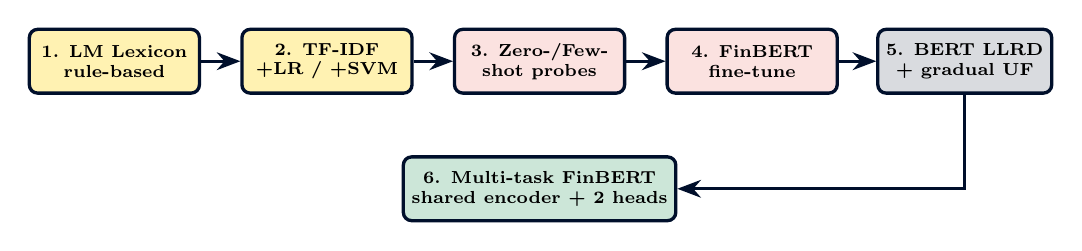
\begin{tikzpicture}[
        box/.style={draw=UNSWDarkBlue, rounded corners=3pt, minimum width=2.4cm, minimum height=0.9cm, align=center, font=\scriptsize\bfseries, line width=1.2pt},
        arr/.style={-{Stealth[length=3mm]}, line width=1.2pt, UNSWDarkBlue},
        scale=0.9, transform shape
    ]
        \node[box, fill=UNSWYellow!30] (s1) at (0, 0) {1. LM Lexicon\\{\scriptsize rule-based}};
        \node[box, fill=UNSWYellow!30] (s2) at (3.0, 0) {2. TF-IDF\\{\scriptsize +LR / +SVM}};
        \node[box, fill=UNSWRed!15] (s3) at (6.0, 0) {3. Zero-/Few-\\{\scriptsize shot probes}};
        \node[box, fill=UNSWRed!15] (s4) at (9.0, 0) {4. FinBERT\\{\scriptsize fine-tune}};
        \node[box, fill=UNSWDarkBlue!15] (s5) at (12.0, 0) {5. BERT LLRD\\{\scriptsize + gradual UF}};
        \node[box, fill=UNSWGreen!20, minimum width=2.8cm] (s6) at (6.0, -1.8) {\textbf{6. Multi-task FinBERT}\\{\scriptsize shared encoder + 2 heads}};

        \draw[arr] (s1) -- (s2);
        \draw[arr] (s2) -- (s3);
        \draw[arr] (s3) -- (s4);
        \draw[arr] (s4) -- (s5);
        \draw[arr] (s5.south) |- (s6.east);
    \end{tikzpicture}

    \vspace{0.6em}
    \begin{itemize}\setlength{\itemsep}{1pt}
        \item Each stage is a \textbf{controlled upgrade} over the previous: add features, add domain prior, add fine-tuning, add training recipe, add multi-task structure.
        \item Every row below is evaluated on the same held-out test sets, so gains are directly comparable.
    \end{itemize}
\end{frame}

% ---- Baselines --------------------------------------------
\begin{frame}{Baselines: Lexicon and TF-IDF}
    \begin{itemize}\setlength{\itemsep}{0.35em}
        \item \textbf{LM Lexicon (rule-based)}~\cite{loughran2011liability} --- count Loughran--McDonald positive/negative terms per sentence, predict by sign. Domain-specific but brittle.
        \item \textbf{TF-IDF + Logistic Regression} --- bigrams (ngram=(1,2)), \texttt{max\_features}=50k, \texttt{sublinear\_tf=True}; LR with default $\ell_2$.
        \item \textbf{TF-IDF + Linear SVM} --- same vectoriser; \texttt{LinearSVC}, $C{=}1.0$, \texttt{class\_weight="balanced"} to offset the neutral skew.
        \item \textbf{TF-IDF (trigrams) + LR} --- richer context: ngram=(1,3), \texttt{max\_features}=80k, \texttt{min\_df}=2.
        \item \textbf{TF-IDF + LM Lexicon (hybrid) + LR} --- concatenate TF-IDF vectors with handcrafted counts of LM positive/negative terms.
    \end{itemize}

    \vspace{0.3em}
    {\small These establish a \textit{domain-aware but shallow} floor. Any neural model we propose must clearly beat them.}
\end{frame}

% ---- Pretrained evaluation --------------------------------
\begin{frame}{Pre-trained Evaluation: Zero-shot and Few-shot}
    \begin{columns}[T]
        \begin{column}{0.50\textwidth}
            \textbf{Zero-shot FinBERT (native 3-way head)}~\cite{araci2019finbert,yang2020finbert}
            \begin{itemize}\setlength{\itemsep}{1pt}
                \item Use the released \{positive, negative, neutral\} head directly on FPB.
                \item For FOMC: \alert{proxy map} positive $\rightarrow$ hawkish, negative $\rightarrow$ dovish, neutral $\rightarrow$ neutral. Tests whether sentiment is a usable proxy for stance.
                \item No parameter updates.
            \end{itemize}
        \end{column}
        \begin{column}{0.48\textwidth}
            \textbf{Few-shot linear probe (k=16 per class)}
            \begin{itemize}\setlength{\itemsep}{1pt}
                \item Freeze encoder, use \texttt{[CLS]} embedding, fit logistic regression on $3\times 16 = 48$ examples.
                \item Compare three frozen backbones:
                \begin{itemize}
                    \item FinBERT (\texttt{ProsusAI/finbert})
                    \item BERT-base-uncased~\cite{devlin2019bert}
                    \item RoBERTa-base
                \end{itemize}
                \item Isolates \textbf{domain pretraining value} in a tiny-data setting.
            \end{itemize}
        \end{column}
    \end{columns}
\end{frame}

% ---- FinBERT ft vs BERT LLRD ------------------------------
\begin{frame}{Fine-tuning: FinBERT vs.\ BERT-base LLRD}
    \begin{columns}[T]
        \begin{column}{0.48\textwidth}
            \begin{block}{FinBERT single-task fine-tune}
                \begin{itemize}\setlength{\itemsep}{1pt}
                    \item Backbone: \texttt{ProsusAI/finbert}
                    \item Optimiser: AdamW, lr $2\mathrm{e}{-5}$, weight decay $0.01$
                    \item Schedule: linear warmup (10\%) + linear decay
                    \item 5 epochs, batch size 32, \texttt{max\_len}=128
                    \item Weighted cross-entropy for FOMC
                    \item Strong domain prior, conventional recipe
                \end{itemize}
            \end{block}
        \end{column}
        \begin{column}{0.48\textwidth}
            \begin{block}{BERT-base LLRD + Gradual Unfreeze~\cite{howard2018ulmfit,sun2019finetune}}
                \begin{itemize}\setlength{\itemsep}{1pt}
                    \item Backbone: \texttt{bert-base-uncased}
                    \item Layer-wise LR decay: head $2\mathrm{e}{-5}$, $\times 0.9$ per depth
                    \item Label smoothing $\varepsilon = 0.1$
                    \item 10 epochs, batch size 32
                    \item Gradual unfreeze: 1 layer group per epoch
                    \item General-purpose backbone, careful recipe
                \end{itemize}
            \end{block}
        \end{column}
    \end{columns}

    \vspace{0.3em}
    {\small The key comparison: does domain pretraining (FinBERT) beat a better \textit{fine-tuning recipe} on a general backbone (BERT-base)? Results say: \textbf{they tie}.}
\end{frame}

% ---- Multi-task architecture ------------------------------
\begin{frame}{Multi-task FinBERT Architecture}
    \begin{columns}[T]
        \begin{column}{0.55\textwidth}
            \centering
            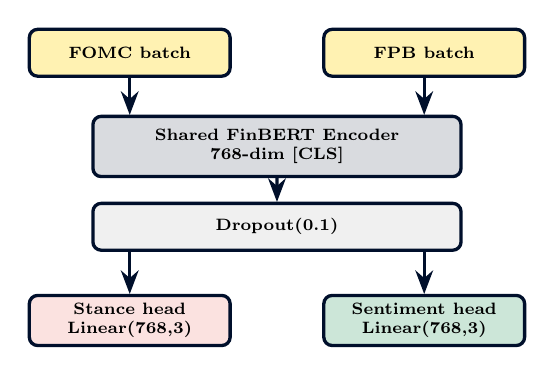
\begin{tikzpicture}[
                box/.style={draw=UNSWDarkBlue, rounded corners=3pt, minimum width=3.0cm, minimum height=0.7cm, align=center, font=\scriptsize\bfseries, line width=1.2pt},
                arr/.style={-{Stealth[length=3mm]}, line width=1.2pt, UNSWDarkBlue},
                scale=0.85, transform shape
            ]
                \node[box, fill=UNSWYellow!30] (inpA) at (-2.2, 4.0) {FOMC batch};
                \node[box, fill=UNSWYellow!30] (inpB) at (2.2, 4.0) {FPB batch};
                \node[box, fill=UNSWDarkBlue!15, minimum width=5.5cm, minimum height=0.9cm] (enc) at (0, 2.6) {\textbf{Shared FinBERT Encoder}\\{\scriptsize 768-dim [CLS]}};
                \node[box, fill=UNSWLightGray, minimum width=5.5cm] (drop) at (0, 1.4) {Dropout(0.1)};
                \node[box, fill=UNSWRed!15] (h1) at (-2.2, 0.0) {Stance head\\{\scriptsize Linear(768,3)}};
                \node[box, fill=UNSWGreen!20] (h2) at (2.2, 0.0) {Sentiment head\\{\scriptsize Linear(768,3)}};

                \draw[arr] (inpA.south) -- (enc.north -| inpA.south);
                \draw[arr] (inpB.south) -- (enc.north -| inpB.south);
                \draw[arr] (enc) -- (drop);
                \draw[arr] (drop.south -| h1.north) -- (h1.north);
                \draw[arr] (drop.south -| h2.north) -- (h2.north);
            \end{tikzpicture}
        \end{column}
        \begin{column}{0.42\textwidth}
            \textbf{Training details}~\cite{liu2019mt-dnn}:
            \begin{itemize}\setlength{\itemsep}{1pt}
                \item \textbf{Alternating batches:} one FOMC batch, then one FPB batch. Each step back-propagates through the shared encoder and the active task's head (the inactive head receives zero gradient).
                \item AdamW, lr $2\mathrm{e}{-5}$, 8 epochs, batch size 32.
                \item Per-task cross-entropy loss (weighted for stance).
                \item \textbf{Best checkpoint} selected by \textit{average} validation macro-F1 across both tasks.
                \item Apple M3 Max (MPS), seed 42.
            \end{itemize}

            \vspace{0.3em}
            {\small Shared encoder $\Rightarrow$ stance examples regularise the sentiment head (and vice versa) --- a free data-augmentation effect.}
        \end{column}
    \end{columns}
\end{frame}

% ============================================================
\section{Results}
% ============================================================

% ---- Baseline results table -------------------------------
\begin{frame}{Baseline \& Lexicon Results}
    \centering
    {\small
    \begin{tabular}{lcccc}
        \toprule
        \textbf{Model} & \textbf{Sent.\ Acc} & \textbf{Sent.\ F1} & \textbf{Stance Acc} & \textbf{Stance F1} \\
        \midrule
        LM Lexicon (rule-based)~\cite{loughran2011liability} & 0.6932 & 0.5315 & 0.4153 & 0.3885 \\
        TF-IDF + LR                                           & 0.8720 & 0.8232 & 0.6089 & 0.5873 \\
        \rowcolor{UNSWYellow!30}
        TF-IDF + SVM (LinearSVC)                              & \textbf{0.8940} & \textbf{0.8534} & \textbf{0.6331} & \textbf{0.6061} \\
        TF-IDF (trigrams) + LR                                & 0.8786 & 0.8310 & 0.6109 & 0.5914 \\
        TF-IDF + LM Lexicon (hybrid) + LR                     & 0.8543 & 0.8050 & 0.6109 & 0.5863 \\
        \bottomrule
    \end{tabular}
    }

    \vspace{0.6em}
    \begin{itemize}\setlength{\itemsep}{1pt}
        \item \textbf{TF-IDF + LinearSVM is the strongest non-neural baseline} on both tasks.
        \item \textbf{Lexicon alone is weak} (FPB F1 only 0.5315, stance F1 0.3885) --- sign-counting cannot handle negation or context.
        \item \textbf{Trigrams give only marginal lift} over bigrams ($+0.66$ pp sentiment, $+0.20$ pp stance accuracy) --- vocabulary grows faster than signal.
        \item Adding LM-lexicon features to TF-IDF does \textit{not} help --- the TF-IDF vocabulary already covers those words.
    \end{itemize}
\end{frame}

% ---- Pretrained results table -----------------------------
\begin{frame}{Pre-trained Models: Zero-shot and Few-shot}
    \centering
    {\small
    \begin{tabular}{lcccc}
        \toprule
        \textbf{Model} & \textbf{Sent.\ Acc} & \textbf{Sent.\ F1} & \textbf{Stance Acc} & \textbf{Stance F1} \\
        \midrule
        FinBERT zero-shot (native head)~\cite{araci2019finbert}    & 0.9735 & 0.9650 & 0.4980 & 0.4874 \\
        \rowcolor{UNSWYellow!30}
        FinBERT few-shot (k=16 probe)                               & \textbf{0.9779} & \textbf{0.9670} & 0.4859 & 0.4534 \\
        BERT-base few-shot (k=16)~\cite{devlin2019bert}             & 0.7417 & 0.6500 & 0.3851 & 0.3744 \\
        RoBERTa-base few-shot (k=16)                                & 0.7682 & 0.6722 & 0.3730 & 0.3600 \\
        \bottomrule
    \end{tabular}
    }

    \vspace{0.6em}
    \begin{itemize}\setlength{\itemsep}{1pt}
        \item \textbf{FinBERT zero-shot is already near-optimal on sentiment} (F1 0.9650) --- its pretraining matches FPB almost exactly.
        \item \textbf{FinBERT dominates both probes}: +30 pp sentiment F1 over BERT/RoBERTa at k=16 --- domain pretraining, not size, is what matters in low-data regimes.
        \item \textbf{Stance is much harder zero-shot}: the positive$\rightarrow$hawkish / negative$\rightarrow$dovish proxy map only reaches F1 0.4874 --- stance $\neq$ sentiment.
        \item The probe tops sentiment but \textit{loses} a little stance F1 vs.\ native head --- 48 examples is too few to learn stance.
    \end{itemize}
\end{frame}

% ---- Fine-tuned results -----------------------------------
\begin{frame}{Fine-tuned Single-Task Models}
    \centering
    {\small
    \begin{tabular}{lcccc}
        \toprule
        \textbf{Model} & \textbf{Sent.\ Acc} & \textbf{Sent.\ F1} & \textbf{Stance Acc} & \textbf{Stance F1} \\
        \midrule
        FinBERT (fine-tuned)                                            & 0.9669 & 0.9459 & 0.6371 & 0.6194 \\
        \rowcolor{UNSWYellow!30}
        BERT-base LLRD + Gradual UF~\cite{howard2018ulmfit,sun2019finetune} & \textbf{0.9757} & \textbf{0.9670} & \textbf{0.6512} & \textbf{0.6383} \\
        \bottomrule
    \end{tabular}
    }

    \vspace{0.6em}
    \begin{itemize}\setlength{\itemsep}{0.3em}
        \item \textbf{BERT-base with LLRD + gradual unfreeze beats single-task FinBERT on both tasks}: $+2.11$ pp sentiment F1 ($0.9459 \!\rightarrow\! 0.9670$) and $+1.89$ pp stance F1 ($0.6194 \!\rightarrow\! 0.6383$); sentiment-F1 ties FinBERT few-shot's $0.9670$.
        \item \textbf{Takeaway:} a disciplined fine-tuning recipe on a general-purpose backbone can close the domain-pretraining gap~\cite{sun2019finetune}.
        \item This is the first evidence in our study that \alert{``domain BERT'' is not the only path} to strong finance-domain results.
    \end{itemize}
\end{frame}

% ---- Multi-task headline ----------------------------------
\begin{frame}{Multi-task FinBERT --- Headline Result}
    \centering
    {\large
    \begin{tabular}{lcc}
        \toprule
                                 & \textbf{Sentiment}         & \textbf{Stance}            \\
        \midrule
        Accuracy                 & \textbf{0.9779}            & \textbf{0.6492}            \\
        Macro-F1                 & \textbf{0.9666}            & \textbf{0.6384}            \\
        \midrule
        $\Delta$ vs.\ single-task FinBERT & \alert{$+2.07$ pp F1} & \alert{$+1.90$ pp F1} \\
        \bottomrule
    \end{tabular}
    }

    \vspace{0.8em}
    \begin{itemize}\setlength{\itemsep}{0.25em}
        \item One shared encoder, two heads, alternating batches --- \textbf{improves both tasks} over single-task FinBERT~\cite{liu2019mt-dnn}.
        \item Sentiment F1 reaches $0.9666$ (matching BERT LLRD's $0.9670$); stance F1 reaches $0.6384$ (within $0.0001$ of BERT LLRD's $0.6383$).
        \item \textbf{Free lunch:} no new data, no new parameters beyond a second 768$\times$3 head, and training cost is comparable to single-task.
    \end{itemize}
\end{frame}

% ---- Full results summary ---------------------------------
\begin{frame}[t]{Results Summary --- All 12 Systems}
    \vspace{-0.5em}
    \centering
    {\footnotesize
    \begin{tabular}{lcccc}
        \toprule
        \textbf{Model} & \textbf{Sent.\ Acc} & \textbf{Sent.\ F1} & \textbf{Stance Acc} & \textbf{Stance F1} \\
        \midrule
        LM Lexicon (rule-based)             & 0.6932 & 0.5315 & 0.4153 & 0.3885 \\
        TF-IDF + LR                         & 0.8720 & 0.8232 & 0.6089 & 0.5873 \\
        TF-IDF + SVM (LinearSVC)            & 0.8940 & 0.8534 & 0.6331 & 0.6061 \\
        TF-IDF (trigrams) + LR              & 0.8786 & 0.8310 & 0.6109 & 0.5914 \\
        TF-IDF + LM Lexicon (hybrid)        & 0.8543 & 0.8050 & 0.6109 & 0.5863 \\
        \midrule
        FinBERT zero-shot (native)          & 0.9735 & 0.9650 & 0.4980 & 0.4874 \\
        FinBERT few-shot (k=16 probe)       & 0.9779 & 0.9670 & 0.4859 & 0.4534 \\
        BERT-base few-shot (k=16)           & 0.7417 & 0.6500 & 0.3851 & 0.3744 \\
        RoBERTa-base few-shot (k=16)        & 0.7682 & 0.6722 & 0.3730 & 0.3600 \\
        \midrule
        FinBERT (fine-tuned)                & 0.9669 & 0.9459 & 0.6371 & 0.6194 \\
        \rowcolor{UNSWYellow!30}
        BERT-base LLRD + Gradual UF         & 0.9757 & \textbf{0.9670} & \textbf{0.6512} & \textbf{0.6383} \textbf{[BEST]} \\
        \rowcolor{UNSWYellow!30}
        \textbf{Multi-task FinBERT}         & \textbf{0.9779} & \textbf{0.9666} & 0.6492 & \textbf{0.6384} \textbf{[BEST]} \\
        \bottomrule
    \end{tabular}
    }

    \vspace{0.4em}
    {\small \textbf{Statistical tie at the top:} Multi-task FinBERT and BERT-base LLRD are \textbf{indistinguishable} within $\pm 0.1$ pp on both macro-F1s. Two very different routes (multi-task + domain backbone vs.\ single-task + careful recipe) reach the same ceiling.}
\end{frame}

% ---- Error analysis ---------------------------------------
\begin{frame}{Error Analysis --- Multi-task FinBERT}
    \begin{columns}[T]
        \begin{column}{0.50\textwidth}
            \textbf{Stance (FOMC test, N=496)}
            \centering
            \vspace{0.2em}

            {\small
            \begin{tabular}{lc}
                \toprule
                \textbf{Class} & \textbf{Per-class F1} \\
                \midrule
                dovish         & 0.6174 \\
                hawkish        & 0.5869 \\
                \rowcolor{UNSWYellow!30}
                neutral        & \textbf{0.7109} \\
                \bottomrule
            \end{tabular}
            }

            \vspace{0.4em}
            {\footnotesize
            \begin{itemize}\setlength{\itemsep}{1pt}
                \item Most errors sit on the \textbf{neutral vs.\ leaning} boundary --- hedged language (``\textit{appropriate to maintain}'') is genuinely ambiguous.
                \item Hawkish is the weakest class (lowest count in train and most lexically diverse).
            \end{itemize}
            }
        \end{column}
        \begin{column}{0.48\textwidth}
            \textbf{Sentiment (FPB test, N=453)}
            \centering
            \vspace{0.2em}

            {\small
            \begin{tabular}{lc}
                \toprule
                \textbf{Class} & \textbf{Per-class F1} \\
                \midrule
                negative       & 0.9500 \\
                \rowcolor{UNSWYellow!30}
                neutral        & \textbf{0.9928} \\
                positive       & 0.9569 \\
                \bottomrule
            \end{tabular}
            }

            \vspace{0.4em}
            {\footnotesize
            \begin{itemize}\setlength{\itemsep}{1pt}
                \item Only \textbf{$\sim 10$ errors total} across 453 test sentences --- sentiment is near-saturated.
                \item Remaining errors are subtle \textit{comparative} constructions (``\textit{profit fell less than expected}'').
            \end{itemize}
            }
        \end{column}
    \end{columns}
\end{frame}

% ============================================================
\section{Analysis}
% ============================================================

% ---- Key findings -----------------------------------------
\begin{frame}{Key Findings}
    \begin{enumerate}\setlength{\itemsep}{0.35em}
        \item \textbf{Stance is a fundamentally harder task than sentiment.} Every model loses $\approx 30$ pp macro-F1 going from FPB to FOMC. The gap is not about data size --- the two datasets are similar --- but about \textit{label pragmatics}.
        \item \textbf{Sentiment is saturated by domain pretraining alone.} FinBERT zero-shot already reaches F1 0.9650; fine-tuning adds almost nothing on FPB. Extra capacity is spent on stance.
        \item \textbf{A careful fine-tuning recipe rivals domain pretraining.} BERT-base with LLRD + gradual unfreeze + label smoothing \textit{beats} single-task FinBERT on both sentiment ($+2.11$ pp) and stance ($+1.89$ pp)~\cite{sun2019finetune,howard2018ulmfit}.
        \item \textbf{Multi-task training is a free lunch.} One shared encoder + two heads improves single-task FinBERT by $+2.07$ pp sentiment F1 and $+1.90$ pp stance F1~\cite{liu2019mt-dnn}, and ties BERT LLRD on both.
        \item \textbf{Zero-shot sentiment $\neq$ stance.} The native FinBERT positive/negative head maps poorly to hawkish/dovish (F1 $0.4874$) --- a reminder that \alert{tone and policy direction are different signals}.
    \end{enumerate}
\end{frame}

% ---- Domain pretraining gap plot --------------------------
\begin{frame}{Domain-Pretraining Gap (k=16 probe)}
    \centering
    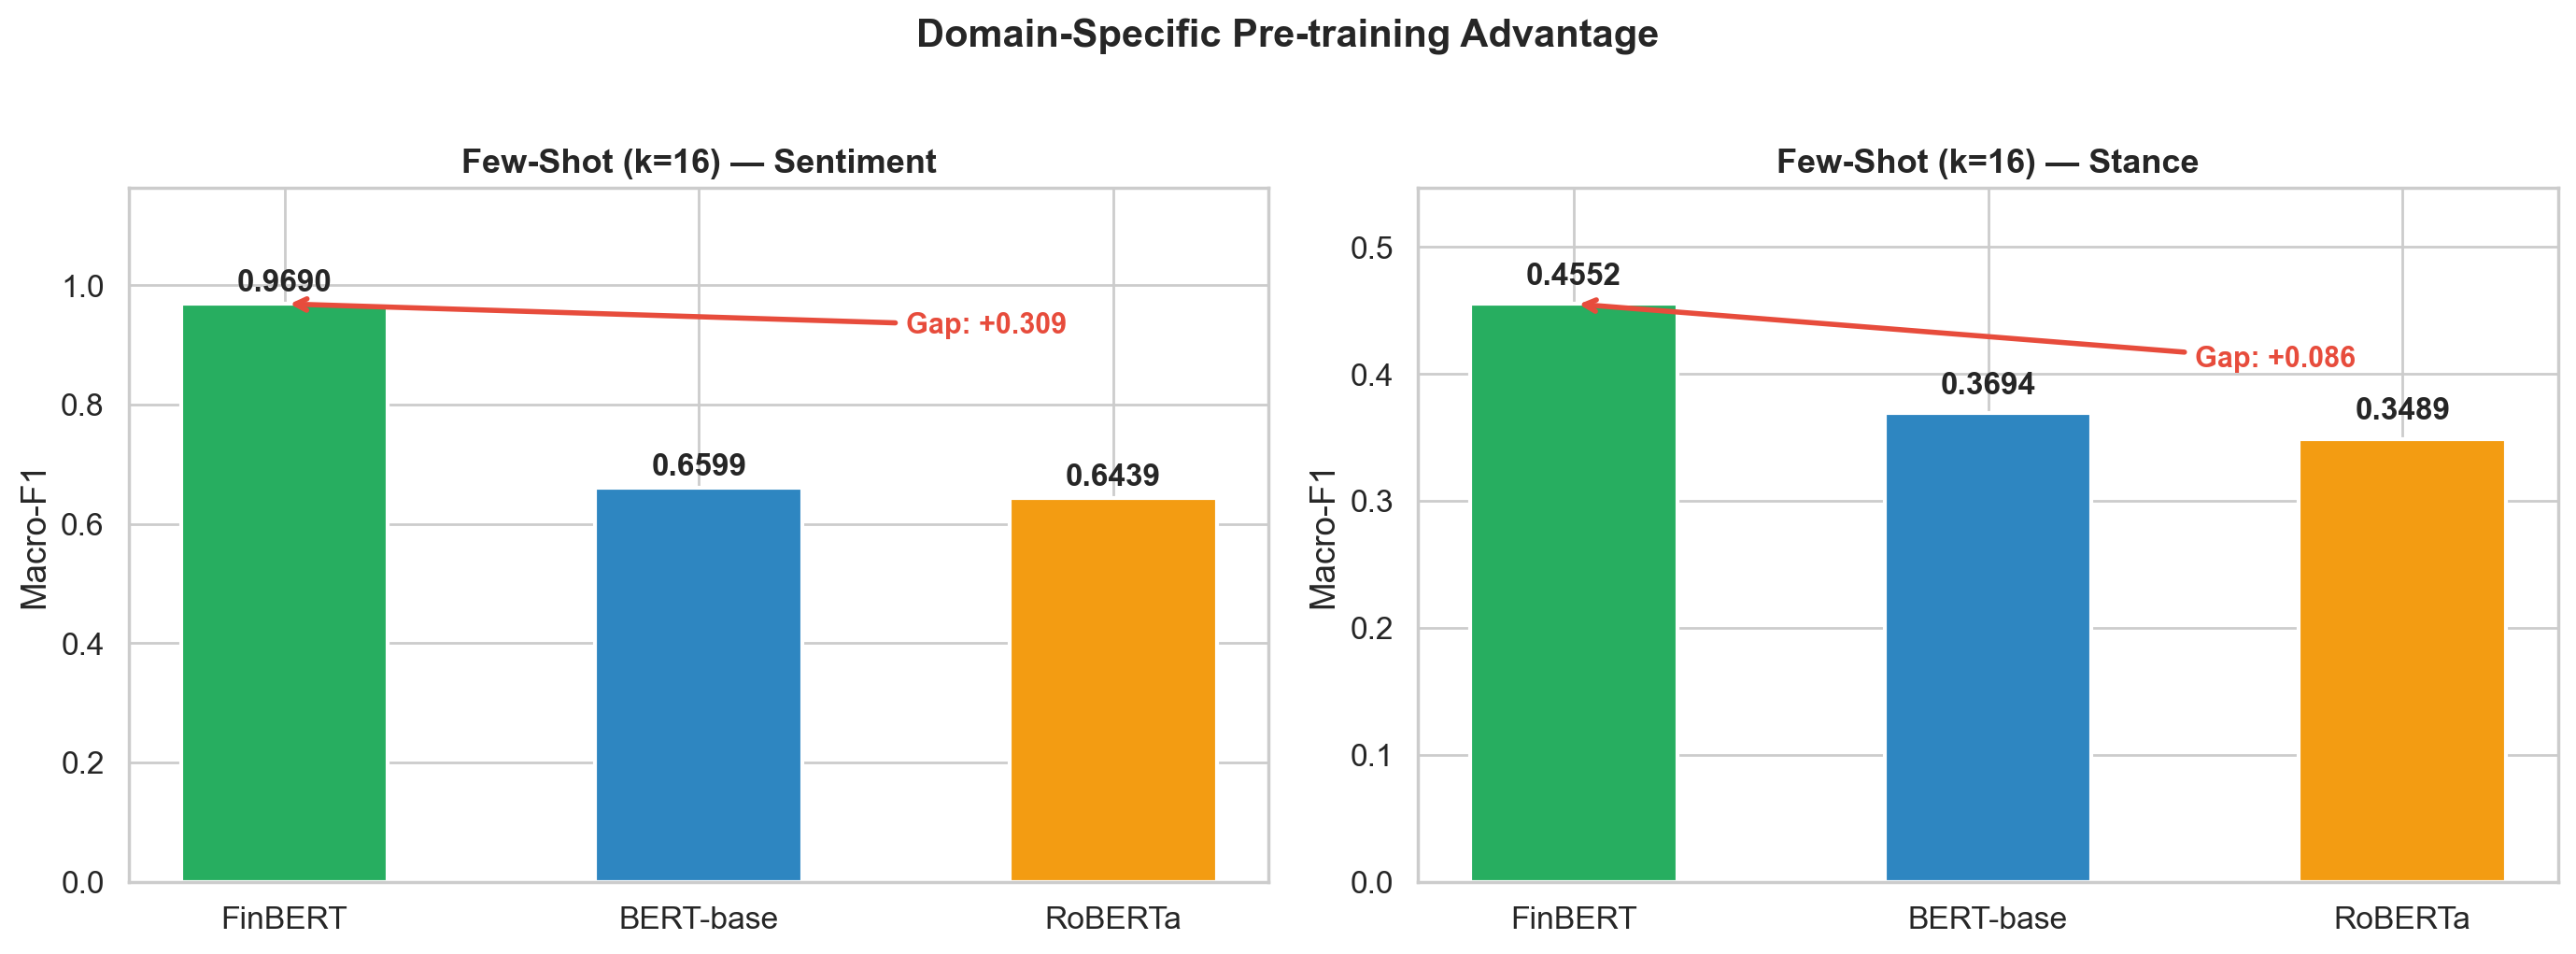
\includegraphics[width=0.72\linewidth]{../analysis/domain_pretraining_gap.png}

    \vspace{0.4em}
    {\small In the low-data regime, \textbf{FinBERT outperforms BERT-base and RoBERTa-base by $\approx 30$ pp sentiment F1}. Fine-tuning closes part of this gap --- but \textit{only} when paired with a careful recipe (LLRD + gradual unfreeze).}
\end{frame}

% ---- Performance progression plot -------------------------
\begin{frame}{Performance Progression Across Methods}
    \centering
    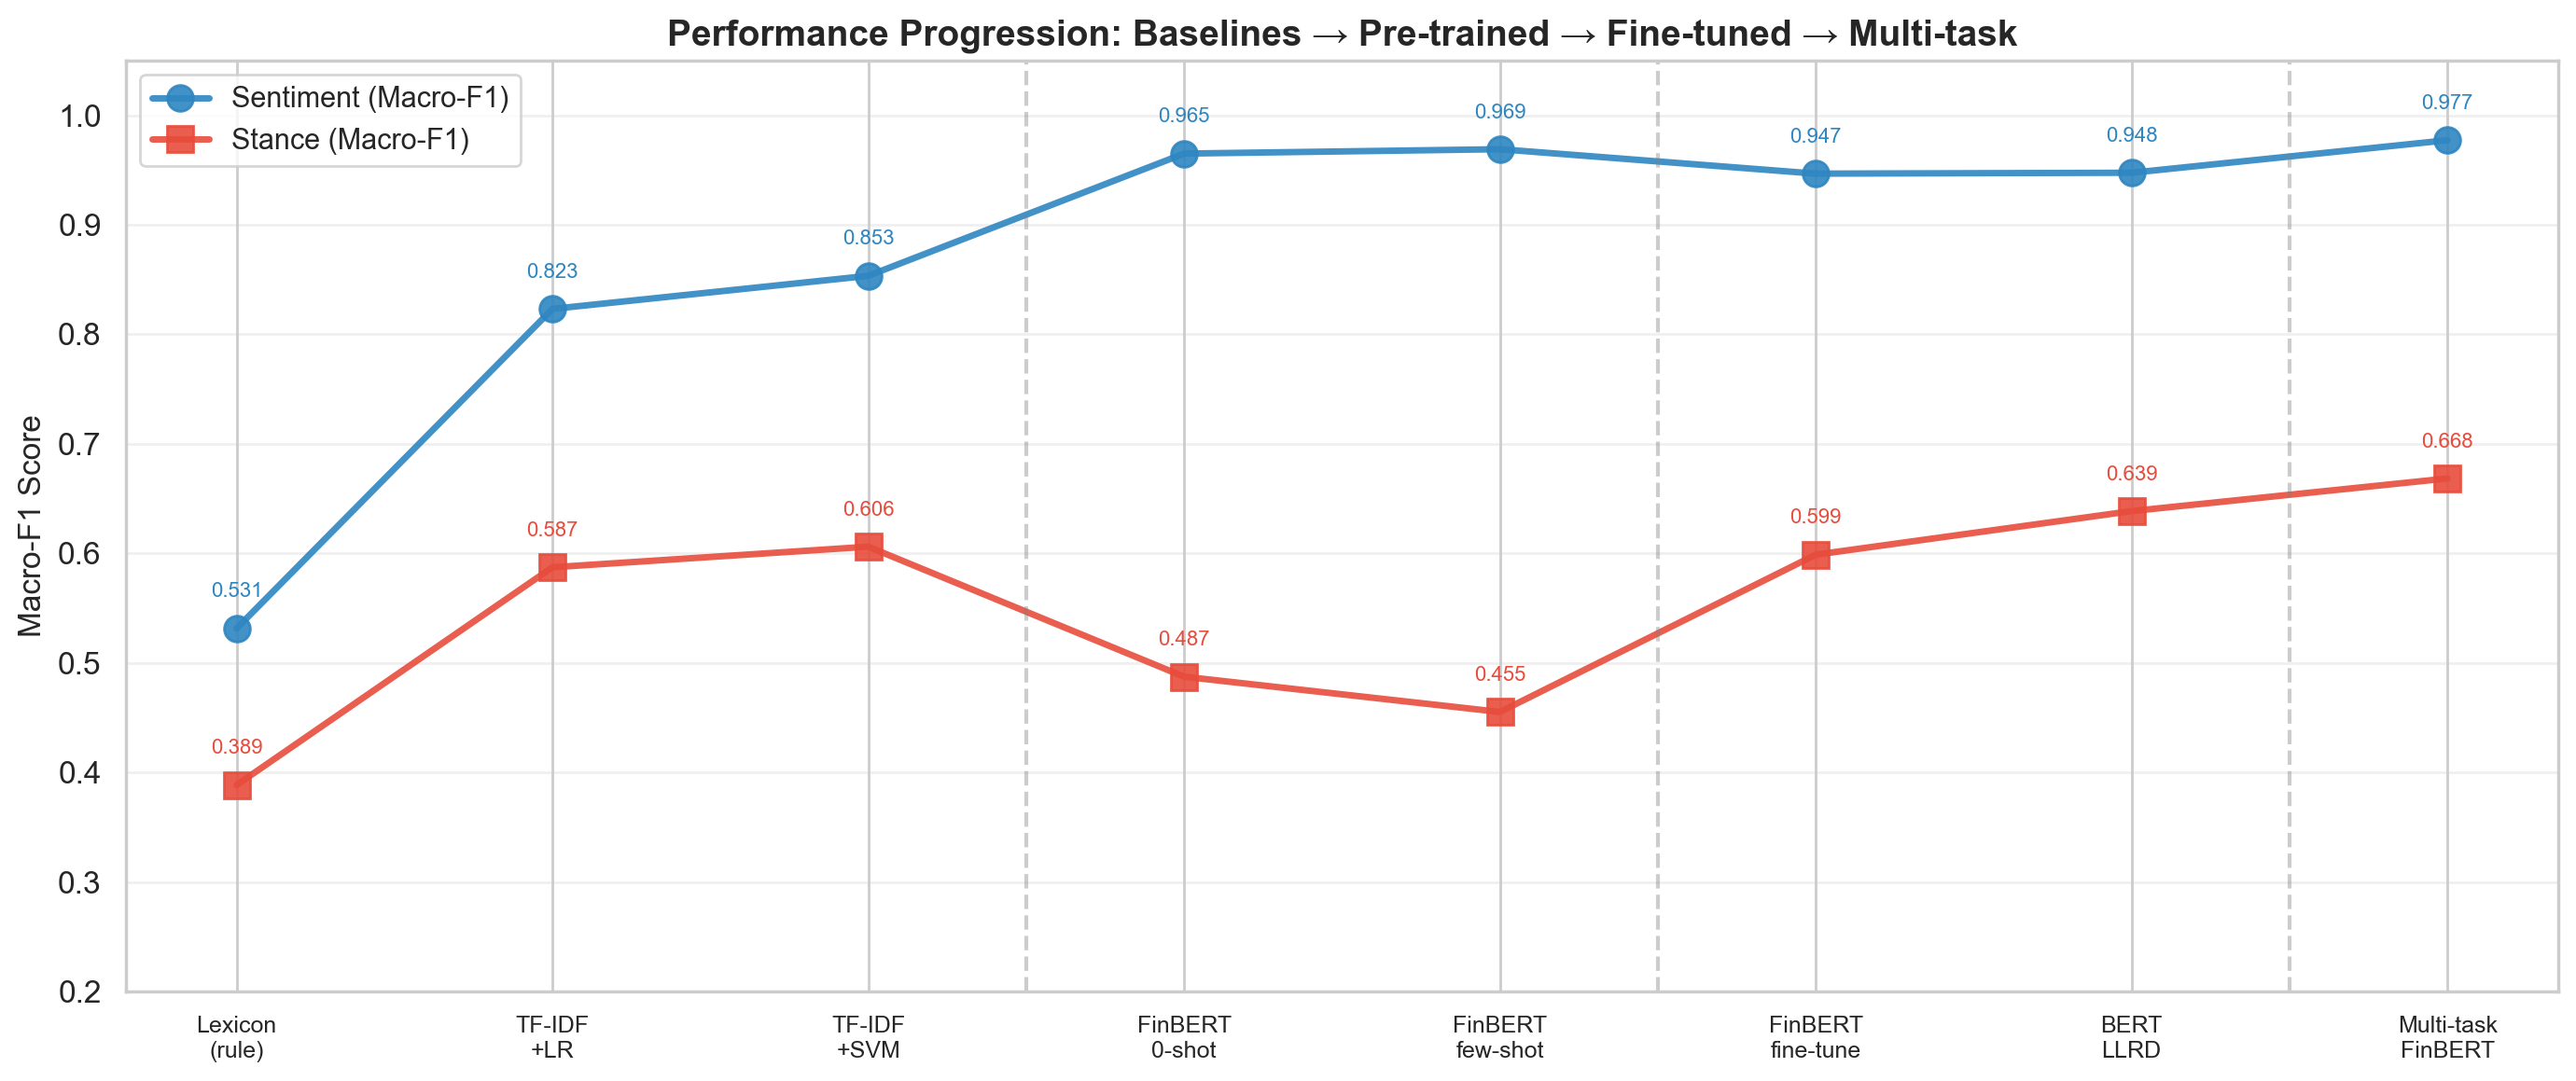
\includegraphics[width=0.78\linewidth]{../analysis/performance_progression.png}

    \vspace{0.2em}
    {\small The sentiment curve \textbf{plateaus} early (FinBERT zero-shot is already near-ceiling); the stance curve keeps climbing through fine-tuning and multi-task. This is where the remaining engineering headroom lies.}
\end{frame}

% ============================================================
\section{Deployment}
% ============================================================

% ---- Deployment slide -------------------------------------
\begin{frame}{Deployment --- CLI, Demo, and Hub Release}
    \begin{columns}[T]
        \begin{column}{0.50\textwidth}
            \textbf{Command-line interface}
            \begin{itemize}\setlength{\itemsep}{1pt}
                \item \texttt{python cli.py --text "The Committee decided to raise the target range."}
                \item Returns predicted stance and sentiment with class probabilities.
                \item Loads the multi-task FinBERT checkpoint by default; single-task checkpoints available via \texttt{--model}.
            \end{itemize}

            \vspace{0.3em}
            \textbf{Interactive demo}
            \begin{itemize}\setlength{\itemsep}{1pt}
                \item Gradio app at \texttt{http://localhost:7860}
                \item Text box + live predictions + per-class probability bars.
                \item Same checkpoint as the CLI --- reproducible.
            \end{itemize}
        \end{column}
        \begin{column}{0.47\textwidth}
            \textbf{HuggingFace Hub release}

            Five public model repos under the \texttt{Louisnguyen/} namespace:
            \begin{itemize}\setlength{\itemsep}{1pt}
                {\scriptsize
                \item \texttt{Louisnguyen/finbert-financial-stance}
                \item \texttt{Louisnguyen/finbert-financial-sentiment}
                \item \texttt{Louisnguyen/bert-llrd-financial-stance}
                \item \texttt{Louisnguyen/bert-llrd-financial-sentiment}
                \item \texttt{Louisnguyen/multitask-finbert-financial}
                }
            \end{itemize}

            \vspace{0.3em}
            {\small Each repo ships weights, tokenizer config, and an inference snippet.}
        \end{column}
    \end{columns}
\end{frame}

% ============================================================
\section{Summary}
% ============================================================

% ---- Summary slide ----------------------------------------
\begin{frame}{Summary}
    \begin{itemize}\setlength{\itemsep}{0.4em}
        \item \textbf{Problem:} joint stance (FOMC) and sentiment (FPB) classification on small, imbalanced financial corpora.
        \item \textbf{Approach:} six-stage progression from LM-lexicon rules through TF-IDF, zero/few-shot probes, single-task fine-tuning (FinBERT and BERT-LLRD), and finally multi-task FinBERT with a shared encoder and two heads.
        \item \textbf{Headline result:} multi-task FinBERT and BERT-base LLRD \textit{tie} for best on both tasks (sentiment F1 $\approx$ 0.967; stance F1 $\approx$ 0.638). Multi-task beats single-task FinBERT by $+2.07$ pp sentiment F1 / $+1.90$ pp stance F1.
        \item \textbf{Lesson:} domain pretraining and careful fine-tuning recipes are \textbf{substitutes}, not complements --- either one reaches the ceiling for this data size.
    \end{itemize}
\end{frame}

% ============================================================
\appendix

% ---- References -------------------------------------------
\begin{frame}[allowframebreaks]{References}
    \printbibliography[heading=none]
\end{frame}

\end{document}
